\documentclass[12pt, a4paper]{report}

% ================= PACKAGES =================
\usepackage[utf8]{inputenc}
\usepackage[T1]{fontenc}
\usepackage[french]{babel}
\usepackage{geometry}
\geometry{top=2.5cm, bottom=2.5cm, left=2.5cm, right=2.5cm}
\usepackage{graphicx}
\usepackage{xcolor}
\usepackage{listings}
\usepackage{hyperref}
\usepackage{fancyhdr}
\usepackage{titlesec}
\usepackage{caption}

% ================= CONFIGURATION =================

% Configuration des liens cliquables
\hypersetup{
    colorlinks=true,
    linkcolor=black,
    filecolor=magenta,      
    urlcolor=blue,
    pdftitle={Rapport Big Data - Détection de Fraude},
}

% Configuration des en-têtes et pieds de page
\pagestyle{fancy}
\fancyhf{}
\rhead{\small \textit{Détection de Fraudes Bancaires - Architecture Lambda}}
\lhead{\small \textit{Big Data / Data Engineering}}
\cfoot{\thepage}

% Configuration de l'affichage du code (Listings)
\definecolor{codegray}{rgb}{0.95,0.95,0.95}
\definecolor{codegreen}{rgb}{0,0.6,0}
\definecolor{codepurple}{rgb}{0.58,0,0.82}
\definecolor{backcolour}{rgb}{0.95,0.95,0.92}

\lstdefinestyle{mystyle}{
    backgroundcolor=\color{backcolour},   
    commentstyle=\color{codegreen},
    keywordstyle=\color{magenta}\bfseries,
    numberstyle=\tiny\color{codegray},
    stringstyle=\color{codepurple},
    basicstyle=\ttfamily\small,
    breakatwhitespace=false,         
    breaklines=true,                 
    captionpos=b,                    
    keepspaces=true,                 
    numbers=left,                    
    numbersep=5pt,                  
    showspaces=false,                
    showstringspaces=false,
    showtabs=false,                  
    tabsize=2,
    frame=single
}

\lstset{style=mystyle}

% ================= DOCUMENT =================

\begin{document}

% ---------------- PAGE DE GARDE ----------------
\begin{titlepage}
    \begin{center}
        \vspace*{1cm}
        
        \Huge
        \textbf{Rapport de Projet Big Data}
        \vspace{0.5cm}
        
        \LARGE
        Data Engineering \& Streaming
        
        \vspace{1.5cm}
        
        \textbf{Sujet :} 
        \vspace{0.5cm}
        
        \huge
        Pipeline de Détection de Fraudes Bancaires en Temps Réel \\
        \vspace{0.2cm}
        \Large
        (Architecture Lambda : Kafka, Spark, HDFS, Impala)
        
        \vspace{2cm}
        
        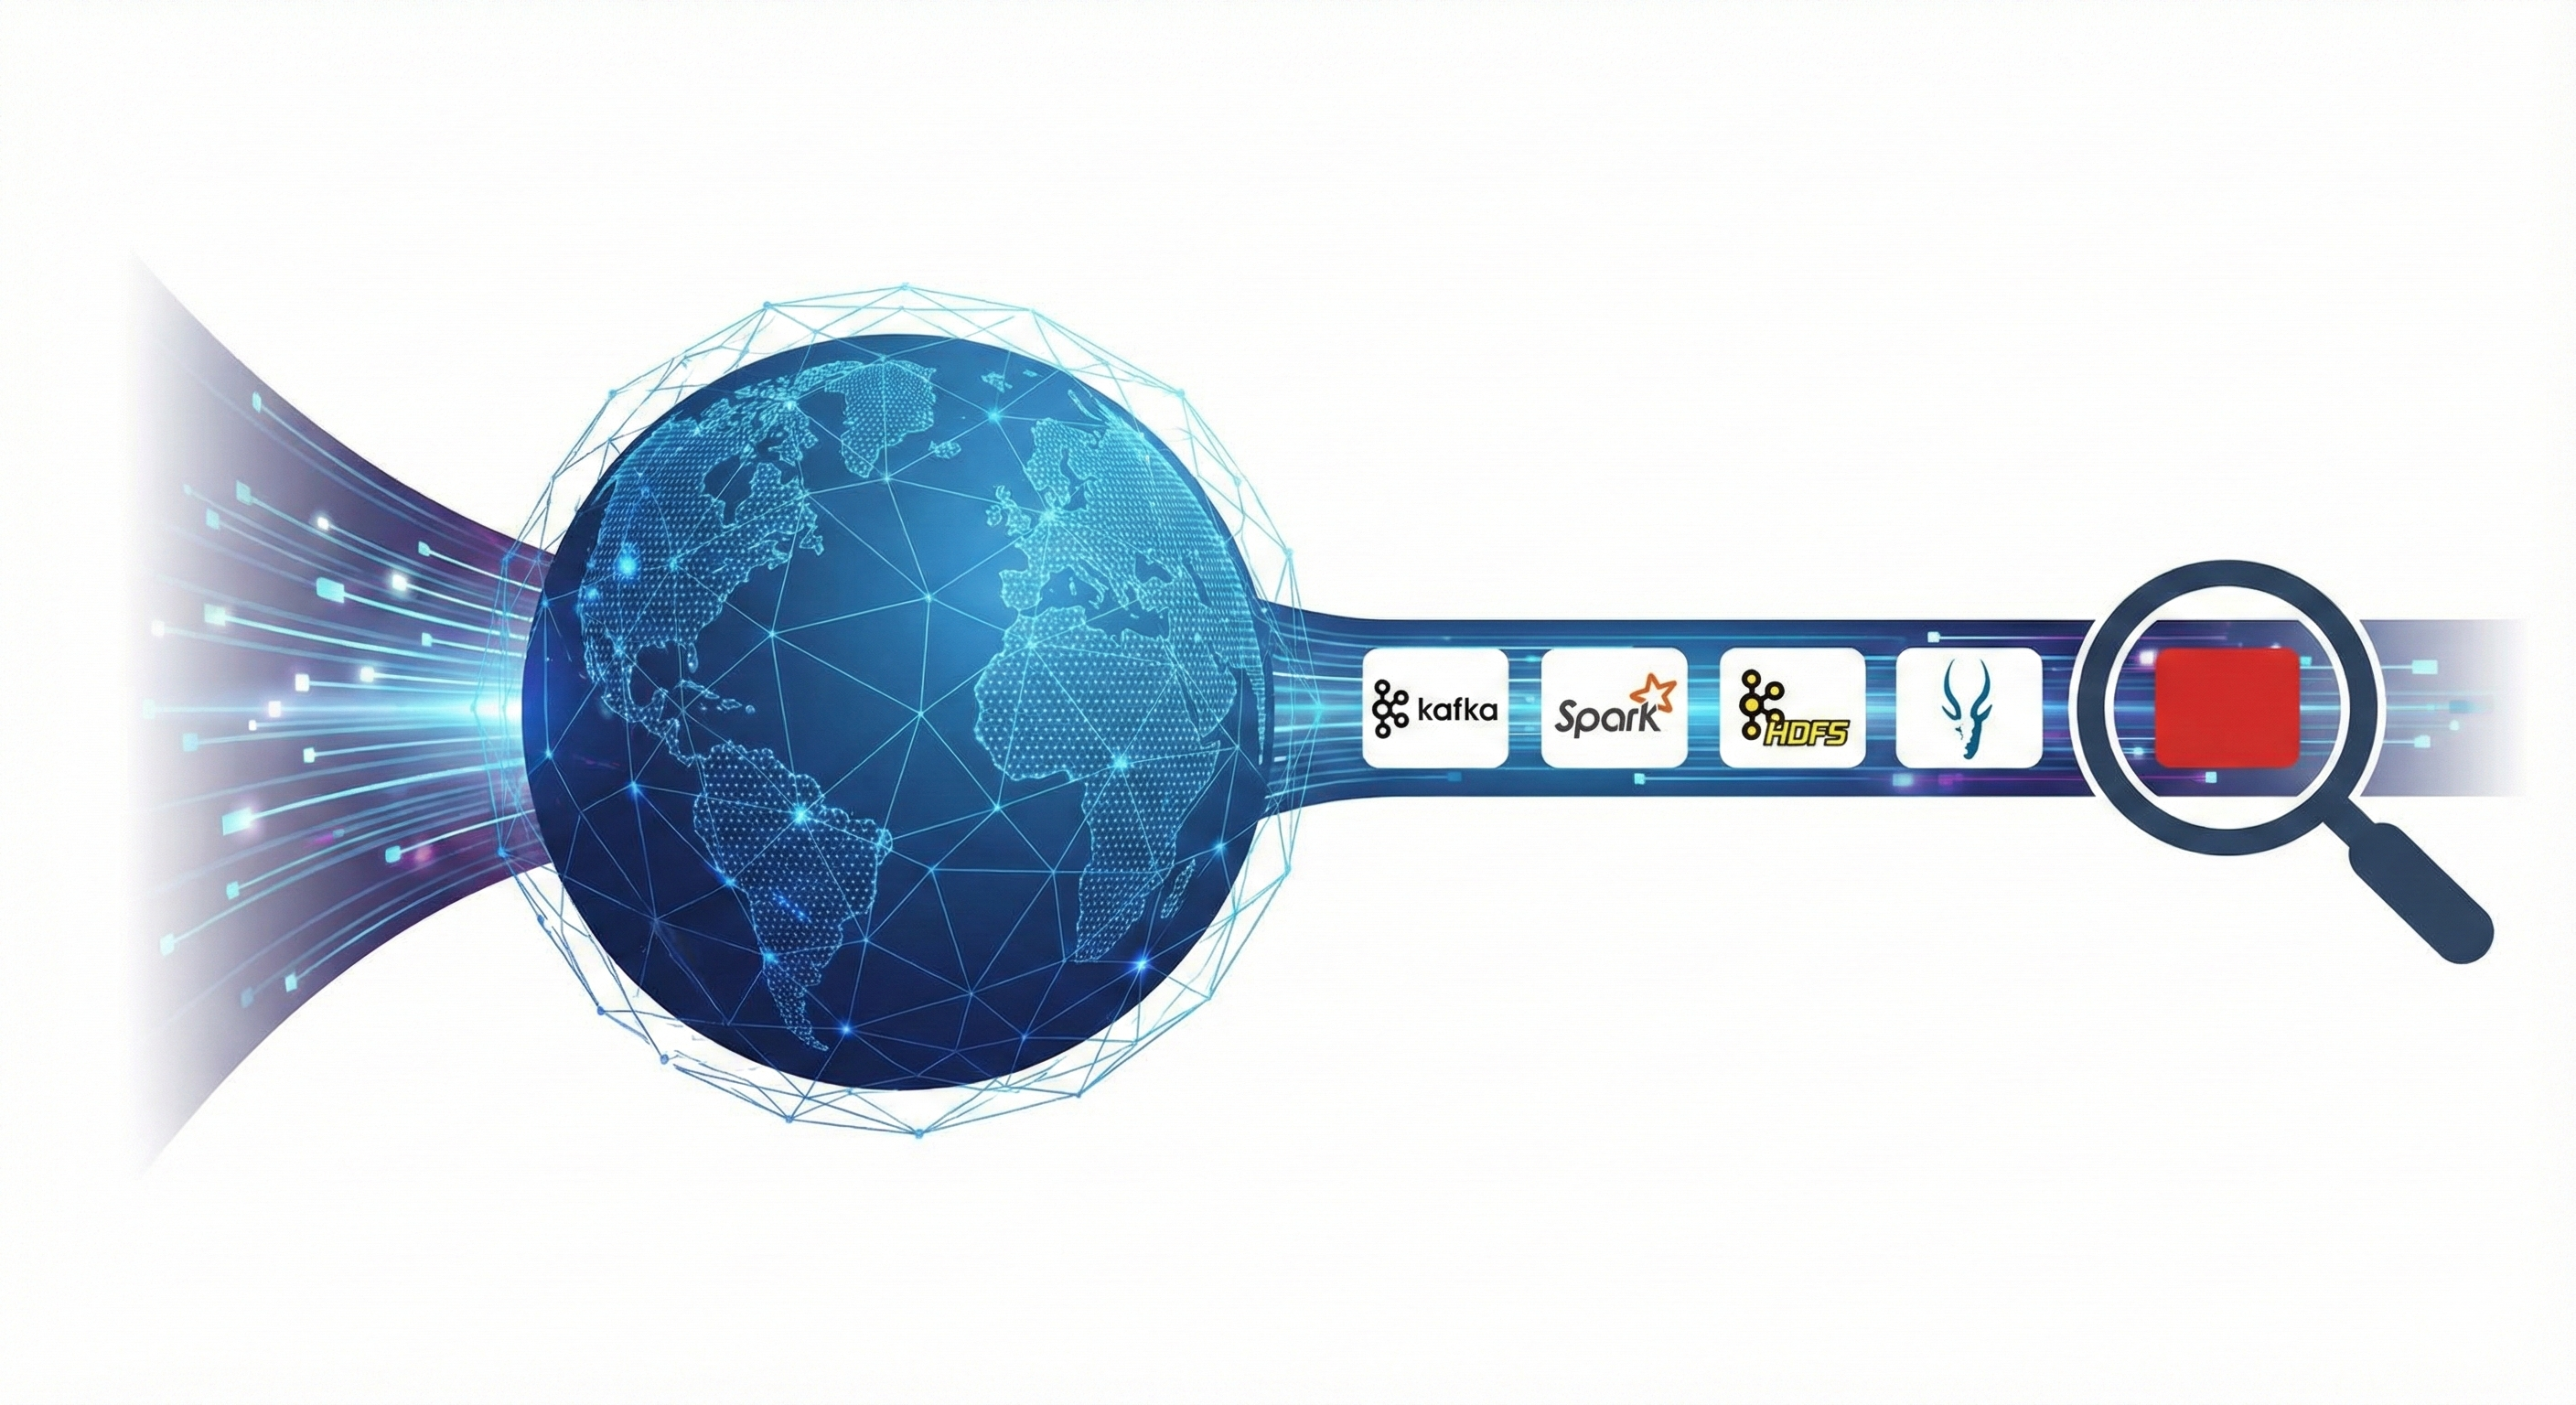
\includegraphics[width=0.6\textwidth]{garde.png} % Placeholder image
        
        \vspace{2cm}
        
        \Large
        \textbf{Réalisé par :} \\
        Mohamed SAKHRI
        
        \vspace{1cm}
        
        \large
        Module : Big Data / Data Engineering \\
        Date : \today
        
    \end{center}
\end{titlepage}

% ---------------- TABLE DES MATIÈRES ----------------
\tableofcontents
\newpage

% ---------------- CHAPITRE 1 : INTRODUCTION ----------------
\chapter{Introduction}

\section{Contexte}
Dans le secteur bancaire moderne, le volume des transactions électroniques croît de manière exponentielle. Les institutions financières font face à un flux continu ("stream") de logs de transactions provenant de terminaux de paiement, de sites e-commerce et d'applications mobiles. Ce flux de données représente une valeur critique mais pose un défi majeur : comment identifier une activité frauduleuse parmi des millions d'opérations légitimes ?

\section{Problématique}
Les méthodes traditionnelles de traitement par lots ("batch processing") sont obsolètes pour la détection de fraude. Attendre la fin de la journée pour analyser les transactions signifie que le fraudeur a déjà disparu avec les fonds.
L'objectif de ce projet est de concevoir un système capable de :
\begin{itemize}
    \item Ingérer des données de transaction en temps réel.
    \item Analyser chaque transaction en moins d'une seconde.
    \item Historiser les données pour des analyses post-mortem.
\end{itemize}

\section{Solution Proposée}
Nous avons implémenté une architecture de type "Lambda", combinant une couche de vitesse ("Speed Layer") pour l'ingestion et le traitement, et une couche de stockage ("Batch Layer") pour l'analyse approfondie. Le pipeline s'appuie sur une stack 100\% Dockerisée utilisant Kafka pour le tampon, Spark Structured Streaming pour le traitement intelligent, HDFS pour le stockage distribué et Impala pour le requêtage SQL interactif.

% ---------------- CHAPITRE 2 : ARCHITECTURE TECHNIQUE DÉTAILLÉE ----------------
\chapter{Architecture Technique Détaillée}

\section{Schéma Global}
Une architecture Big Data robuste repose sur la séparation des responsabilités. Le schéma ci-dessous illustre le flux de données complet, de la génération à la visualisation.

\begin{figure}[h]
    \centering
    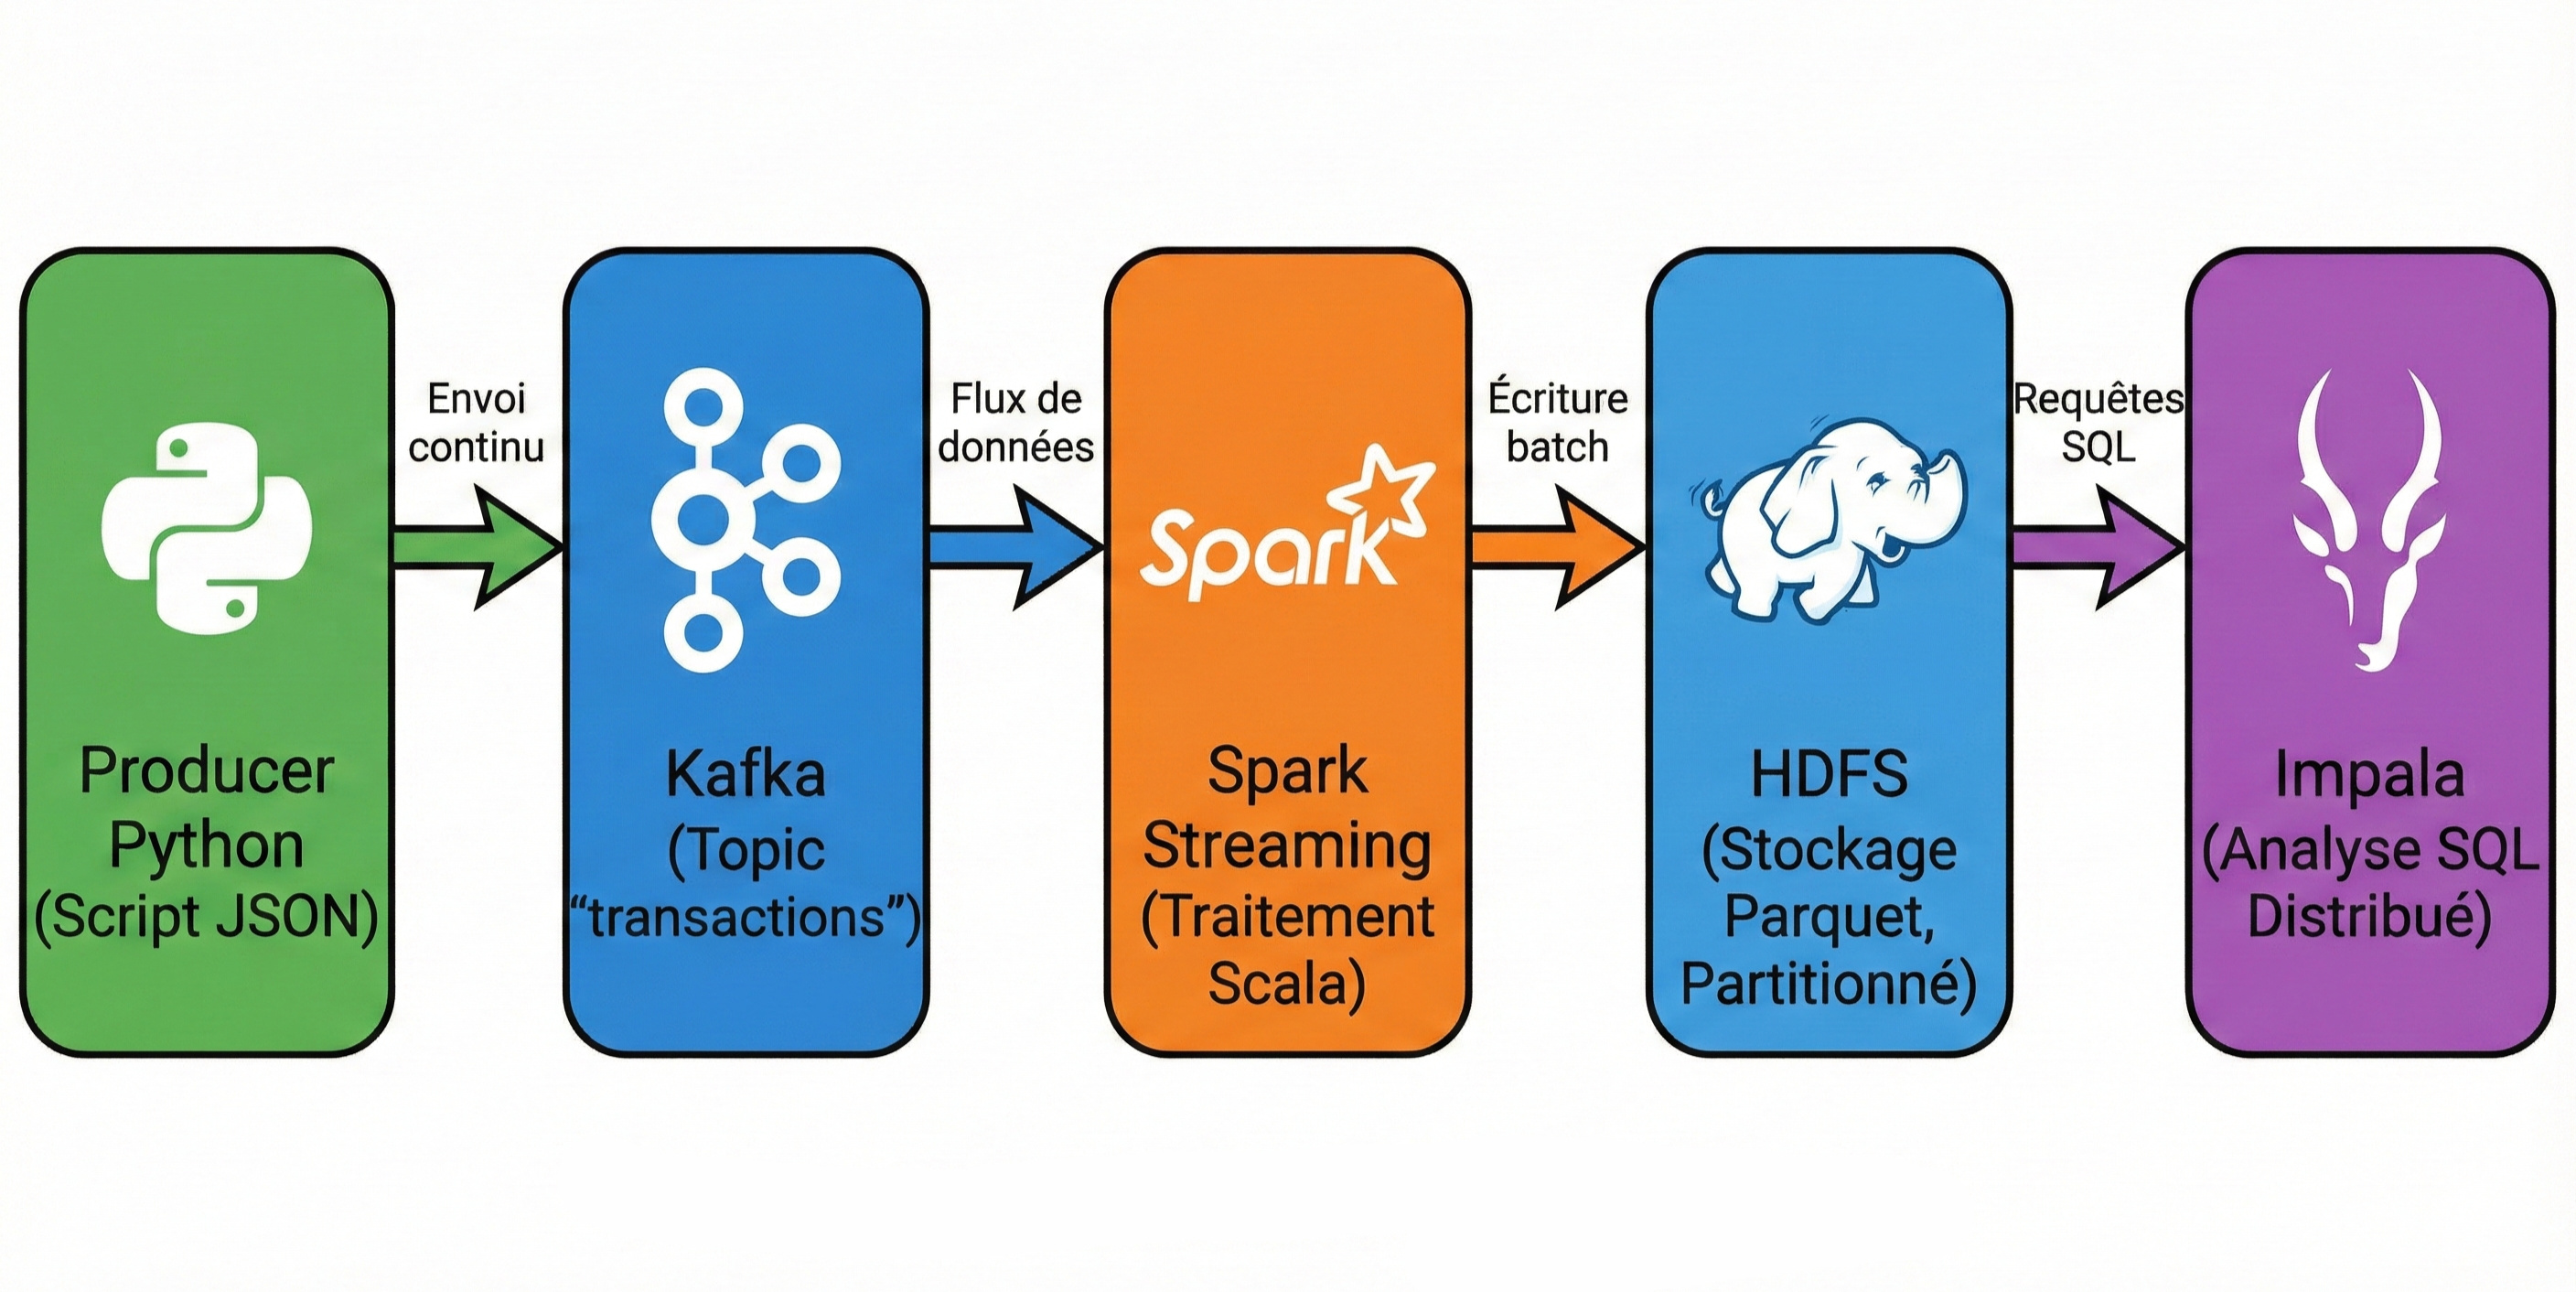
\includegraphics[width=1\textwidth]{workflow.png} % Placeholder GRAND
    \caption{Architecture Lambda : Speed Layer (Spark) et Batch Layer (HDFS/Impala)}
    \label{fig:architecture}
\end{figure}

Le pipeline se décompose en 4 étapes majeures :
\begin{enumerate}
    \item \textbf{Ingestion} : Un producer Python génère des transactions aléatoires JSON et les publie dans Kafka.
    \item \textbf{Processing} : Spark Structured Streaming lit Kafka, applique des règles métier (Fraude > 10k), et écrit en Parquet.
    \item \textbf{Stockage} : HDFS (Hadoop Distributed File System) stocke les fichiers Parquet de manière distribuée et partitionnée.
    \item \textbf{Serving} : Impala offre une vue SQL sur ces fichiers pour l'analyse BI.
\end{enumerate}

\section{Infrastructure Dockerisée}
L'ensemble du projet tourne sur une stack Docker Compose interconnectée via un réseau bridge `bigdata-network`.

\subsection{Configuration des Services (Docker Compose)}
Voici un extrait critique de notre fichier `docker-compose.yml` montrant la définition du service Spark Master et Impala.

\begin{lstlisting}[language=yaml, caption=Extrait du docker-compose.yml]
version: '2'
services:
  # --- Message Broker ---
  kafka:
    image: wurstmeister/kafka:latest
    ports:
      - "9092:9092"
    environment:
      KAFKA_ADVERTISED_LISTENERS: INSIDE://kafka:9093,OUTSIDE://localhost:9092
      KAFKA_LISTENERS: INSIDE://0.0.0.0:9093,OUTSIDE://0.0.0.0:9092
      KAFKA_LISTENER_SECURITY_PROTOCOL_MAP: INSIDE:PLAINTEXT,OUTSIDE:PLAINTEXT
      KAFKA_INTER_BROKER_LISTENER_NAME: INSIDE

  # --- Processing Engine ---
  spark-master:
    image: apache/spark:3.5.0
    container_name: spark-master
    ports:
      - "8080:8080"
      - "7077:7077"
    command: ["/opt/spark/bin/bin/spark-class", "org.apache.spark.deploy.master.Master"]

  # --- SQL Engine ---
  impala:
    image: apache/kudu:impala-latest
    command: ["impala"]
    environment:
      - KUDU_MASTERS= # Désactive la dépendance Kudu
    ports:
      - "21000:21000" # Thrift Server (JDBC/ODBC)
      - "25010:25010" # Web UI
\end{lstlisting}

\begin{figure}[h]
    \centering
    \includegraphics[width=0.9\textwidth]{docker_up.png} 
    \caption{État des conteneurs}
    \label{fig:docker_ps}
\end{figure}

\section{Justification Approfondie des Choix}

\subsection{Pourquoi le format Parquet ?}
Contrairement au CSV (basé ligne) ou au JSON (verbeux), Parquet est un format "colonnaire".
\begin{itemize}
    \item \textbf{Projection Pushdown} : Impala peut lire uniquement la colonne `montant` sans lire `ville` ou `id`, réduisant les I/O disque de 90\%.
    \item \textbf{Compression} : Les valeurs d'une même colonne se ressemblent souvent (ex: "France", "France"...), permettant une compression RLE très efficace.
    \item \textbf{Typage} : Le schéma est embarqué, évitant les erreurs de parsing à la lecture.
\end{itemize}

% ---------------- CHAPITRE 3 : IMPLÉMENTATION ----------------
\chapter{Implémentation du "Cœur" Technique}

\section{Ingestion des Données (Python)}
Le script `producer.py` utilise la librairie `kafka-python-ng` pour simuler un trafic bancaire réaliste.

\begin{lstlisting}[language=Python, caption=Génération de données (producer.py)]
# Simulation de données variées
villes = ["Paris", "Lyon", "Marseille", "Bordeaux", "Lille"]
types = ["CB", "Virement", "Ligne", "Retrait"]

transaction = {
    "id": random.randint(1000, 9999),
    "montant": random.uniform(10.0, 15000.0), 
    "ville": random.choice(villes),
    "type": random.choice(types),
    "timestamp": int(time.time())
}
# Envoi au topic 'transactions'
producer.send('transactions', value=transaction)
\end{lstlisting}

\begin{figure}[h]
    \centering
    \includegraphics[width=1\textwidth]{python.png}
    \caption{Console Ingestion : Logs montrant l'envoi des messages en temps réel}
    \label{fig:ingestion}
\end{figure}
\newpage
\section{Traitement Spark Structured Streaming (Scala)}
C'est le cœur du système. Nous utilisons l'API `DataStreamReader` de Spark.

\subsection{Lecture du Flux Kafka}
\begin{lstlisting}[language=Scala]
val kafkaDF = spark.readStream
  .format("kafka")
  .option("kafka.bootstrap.servers", "kafka:9093") 
  .option("subscribe", "transactions")
  .load()
\end{lstlisting}

\subsection{Logique Métier et Partitionnement}
Le partitionnement est la clé de la performance. En partitionnant par `ville`, nous créons des sous-dossiers physiques.

\begin{lstlisting}[language=Scala, caption=Écriture sur HDFS avec Partitionnement]
    // 5. Écriture dans HDFS
    val query = processedDF.writeStream
      .format("parquet")
      .option("path", "hdfs://namenode:8020/user/hive/warehouse/transactions")
      .option("checkpointLocation", "/tmp/checkpoints/transactions")
      .partitionBy("ville") // Création de dossiers ville=Paris/ etc.
      .outputMode("append")
      .start()
\end{lstlisting}

\begin{figure}[h]
    \centering
    \includegraphics[width=1\textwidth]{spark_UI.png}
    \caption{Interface Spark UI : le job de Streaming actif}
    \label{fig:spark_ui}
\end{figure}

% ---------------- CHAPITRE 4 : DÉPLOIEMENT ET GUIDE D'USAGE ----------------
\chapter{Guide de Déploiement et Utilisation}

Ce chapitre détaille les étapes pour reproduire le projet de A à Z.

\section{Démarrage de l'Infrastructure}
Il faut d'abord lancer les conteneurs. Nous utilisons le mode "détaché".
\begin{lstlisting}[language=bash]
docker compose up -d
\end{lstlisting}
Cette commande initialise Zookeeper, Kafka, les Datanodes HDFS, Spark Master/Worker et Impala.

\section{Lancement de l'Ingestion}
Dans un terminal dédié, nous lançons le script d'ingestion qui prépare l'environnement Python et lance le producer.
\begin{lstlisting}[language=bash]
./start_ingestion.sh
\end{lstlisting}

\section{Soumission du Job Spark}
Le script `submit\_job.sh` est critique. Il compile le code Scala avec SBT (encapsulé dans Docker) et soumet le JAR au cluster Spark.
\begin{lstlisting}[language=bash]
./submit_job.sh refresh
\end{lstlisting}
L'argument `refresh` permet de nettoyer les checkpoints HDFS pour repartir de zéro (très utile en développement).

\begin{figure}[h]
    \centering
    \includegraphics[width=1\textwidth]{submetting_job.png}
    \caption{Compilation SBT réussie et soumission au cluster}
    \label{fig:compilation}
\end{figure}

% ---------------- CHAPITRE 5 : DIFFICULTÉS ET SOLUTIONS ----------------
\chapter{Problèmes Rencontrés et Solutions}

Le développement d'un tel pipeline sur Windows avec Docker comporte des pièges spécifiques.

\section{Le Problème des Chemins HDFS sur Windows (Git Bash)}
\textbf{Symptôme :} Les commandes `hdfs dfs -ls /` échouaient avec une erreur `No FileSystem for scheme "C"`.
\\
\textbf{Cause :} Git Bash sur Windows tente de convertir le chemin absolu `/` en chemin Windows `C:/Program Files/Git/`, ce que le client HDFS Dockerisé ne comprend pas.
\\
\textbf{Solution :} Nous avons utilisé deux stratégies :
\begin{enumerate}
    \item L'utilisation du double slash `//` (ex: `//user/hive/...`) pour échapper la conversion automatique.
    \item L'utilisation systématique de l'URI complète `hdfs://namenode:8020/...` qui est non-ambiguë.
\end{enumerate}

\section{Instabilité du Conteneur Impala}
\textbf{Symptôme :} Le conteneur `impala` démarrait et s'arrêtait immédiatement ("Exited").
\\
\textbf{Cause :} L'image `apache/kudu:impala-latest` est par défaut configurée pour chercher un master Kudu. N'ayant pas déployé Kudu, le processus `impalad` échouait au démarrage. De plus, tenter de surcharger l'`entrypoint` causait des erreurs de librairies partagées (`libjvm.so not found`).
\\
\textbf{Solution :} Nous avons identifié qu'il fallait désactiver la recherche de master Kudu via une variable d'environnement vide et laisser l'entrypoint par défaut faire son initialisation de chemins.
\begin{lstlisting}[language=yaml]
environment:
  - KUDU_MASTERS=  # Laisser vide corrige le crash
\end{lstlisting}

\section{Conflit de Métadonnées `\_spark\_metadata`}
\textbf{Symptôme :} Impala refusait de lire la table ou affichait des erreurs de format.
\\
\textbf{Cause :} Spark streaming écrit ses logs de transaction dans un dossier `\_spark\_metadata` à la racine. Impala essayait de lire ce dossier comme une partition de données.
\\
\textbf{Solution :} L'usage de `.partitionBy("ville")` a déplacé les données réelles dans des sous-dossiers (ex: `ville=Paris`), permettant à Impala d'ignorer proprement la racine polluée via la commande `RECOVER PARTITIONS`.

% ---------------- CHAPITRE 6 : ANALYSE DES RÉSULTATS ----------------
\chapter{Analyse des Résultats (Impala)}

L'étape finale consiste à interroger les données.

\section{Requêtes SQL Analytiques}

\subsection{Création de la Table}
\begin{lstlisting}[language=SQL]
CREATE EXTERNAL TABLE transactions_fraude (
    id INT,
    montant DOUBLE,
    `type` STRING,
    `timestamp` BIGINT,
    is_fraud BOOLEAN
)
PARTITIONED BY (ville STRING)
STORED AS PARQUET
LOCATION 'hdfs://namenode:8020/user/hive/warehouse/transactions';
\end{lstlisting}

\subsection{Récupération des Partitions}
\begin{lstlisting}[language=SQL]
ALTER TABLE transactions_fraude RECOVER PARTITIONS;
\end{lstlisting}
\textit{Cette commande est essentielle : elle informe Impala que de nouveaux dossiers (villes) sont apparus sur HDFS.}

\section{Tableau de Bord KPI}

\begin{figure}[!h]
    \centering
    \includegraphics[width=1\textwidth]{SQL.png}
    \caption{ Exécution des requêtes SQL et résultats tabulaires}
    \label{fig:impala_result}
\end{figure}

Les résultats montrent clairement les villes les plus touchées :

\begin{lstlisting}[language=SQL]
SELECT ville, count(*) as nb_fraudes
FROM transactions_fraude WHERE is_fraud=true GROUP BY ville;
\end{lstlisting}

\textbf{Interprétation :} Si Paris apparaît en tête, cela corrèle avec le volume de transactions plus élevé simulé par notre script Python.

% ---------------- CHAPITRE 7 : CONCLUSION ----------------
\chapter{Conclusion}

Ce projet a permis de valider une chaîne de traitement complète "End-to-End".
Nous avons réussi à :
\begin{itemize}
    \item Mettre en place un environnement distribué complexe sur une machine locale de développement.
    \item Résoudre des problèmes d'intégration délicats (Réseau Docker, Compatibilité Windows/Linux).
    \item Produire des indicateurs métier (KPI) exploitables à partir de données brutes.
\end{itemize}

Les perspectives d'évolution incluraient l'ajout d'une interface de visualisation type "Grafana" ou "Superset" branchée directement sur Impala via JDBC, pour offrir des tableaux de bord en temps réel aux décideurs.

\end{document}
